\section{Empirical Evaluation}
%- resultados basicos segun los distintos encodings
%- resultados comparativos de cuando empiezan a fallar en mapas cuadrados vacios
%- analisis varios (porq el encoding mejora o empeora)
%- hablar de cosas negativas
%- empezar a ver una cota tentativa segun numero de celdas.

%- comparar cambiar restricciones del dijkstra. Un problema en grilla cuadrada.
%- usar la version mas simple.

\begin{figure*}
    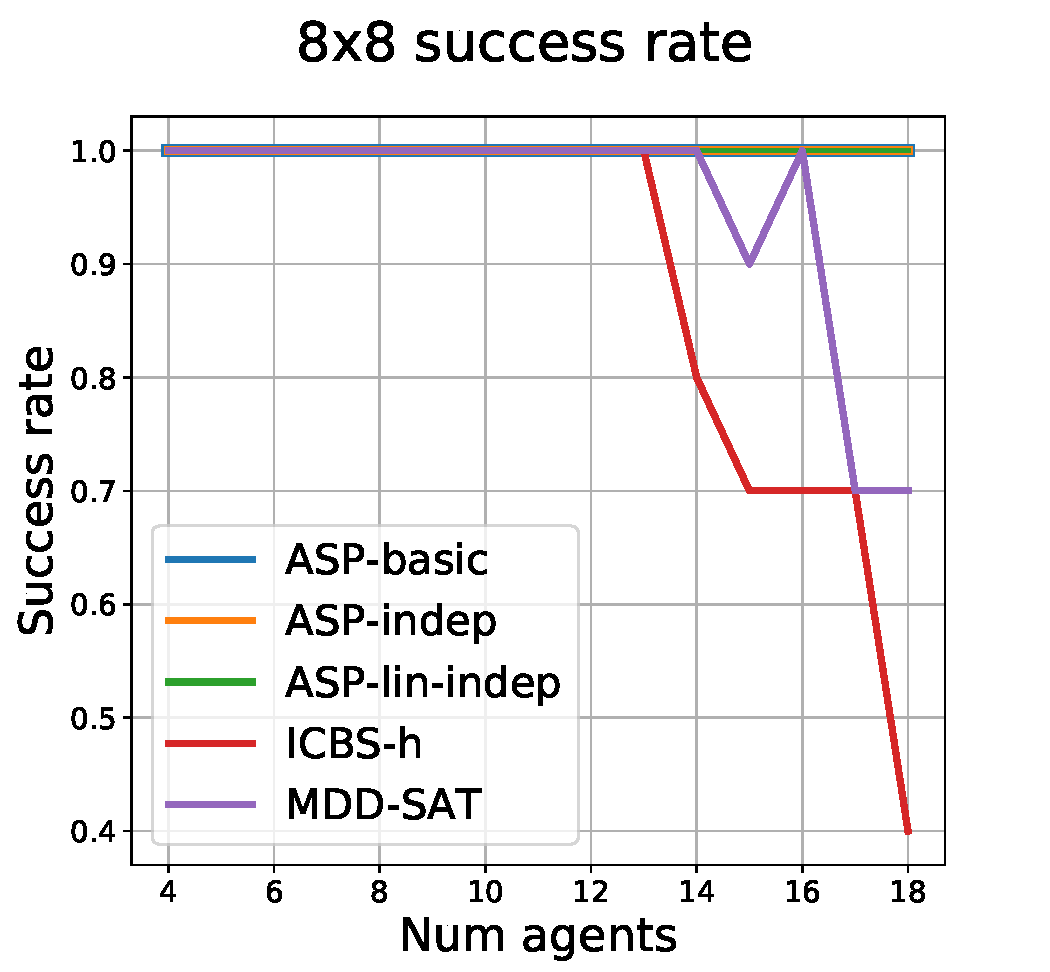
\includegraphics[width=0.24\textwidth]{graphs/8x8succ.pdf}
    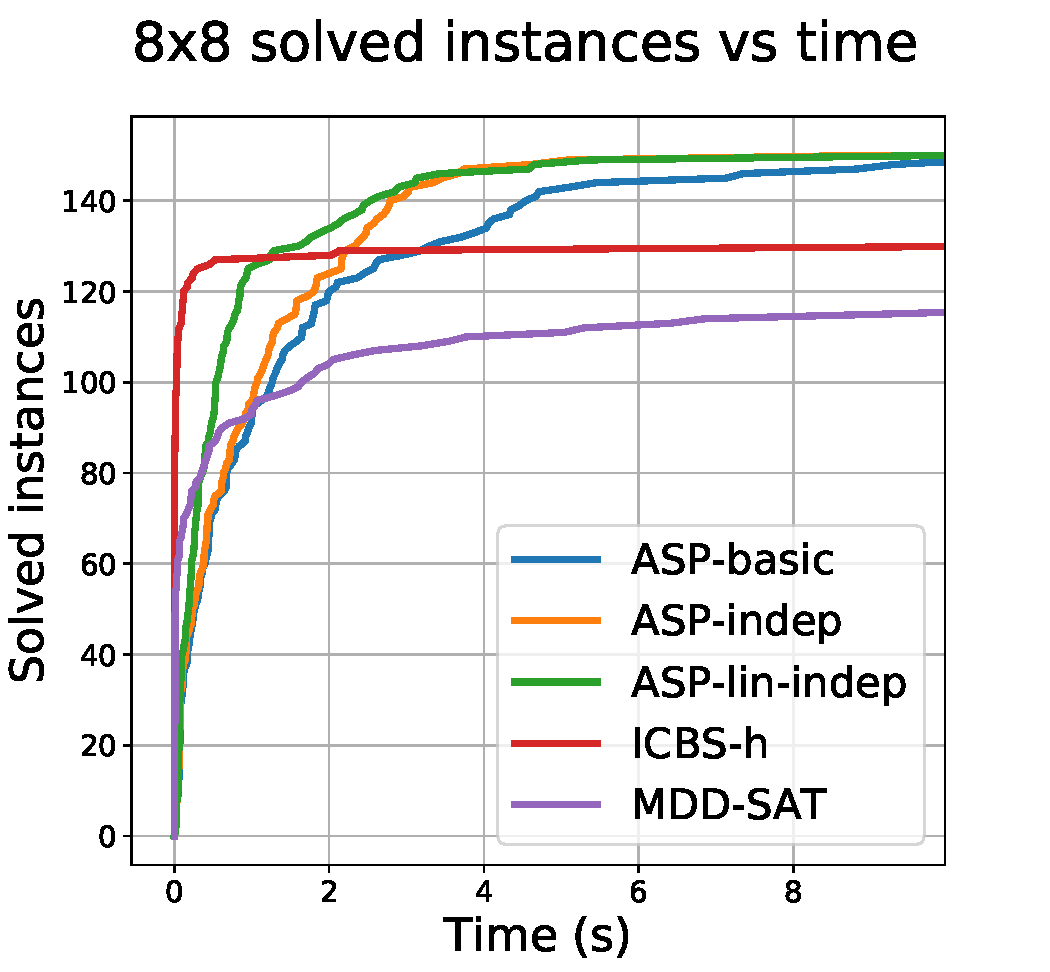
\includegraphics[width=0.24\textwidth]{graphs/8x8runtime.pdf}
    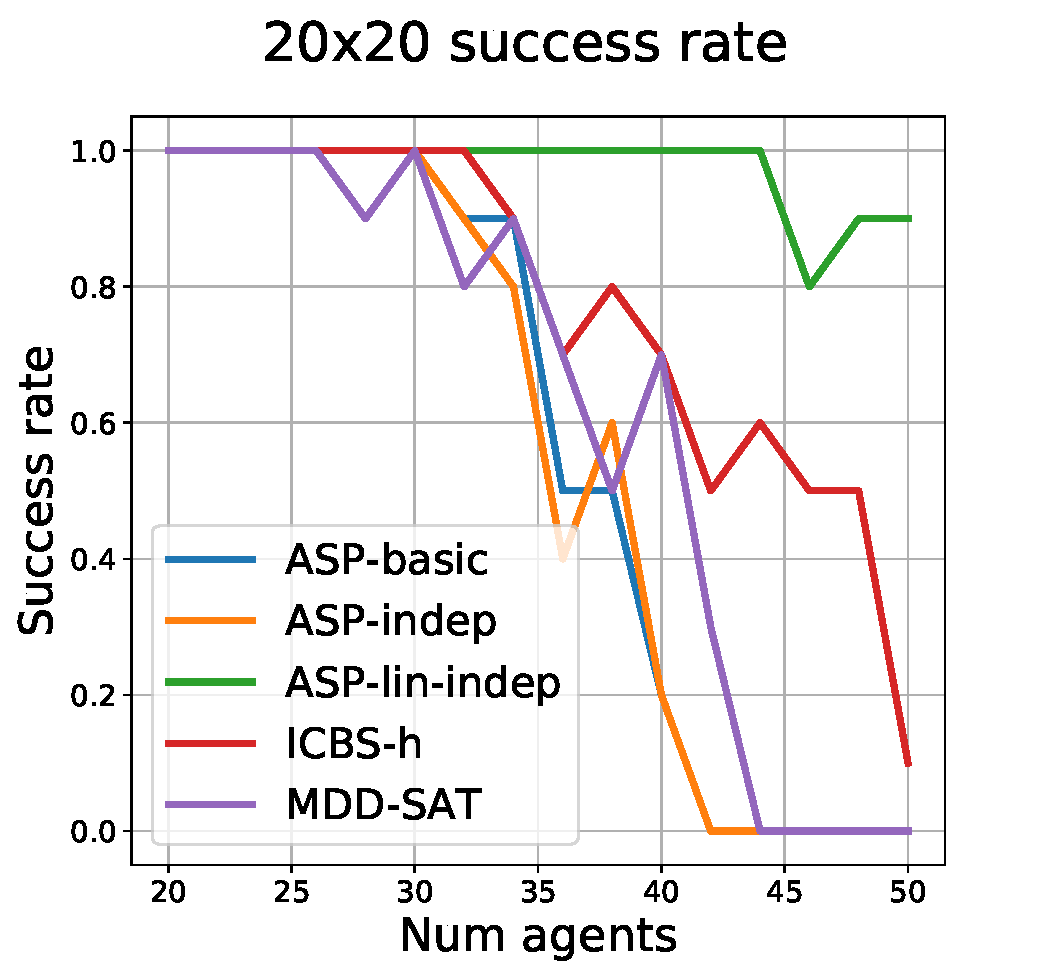
\includegraphics[width=0.24\textwidth]{graphs/20x20succ.pdf}
    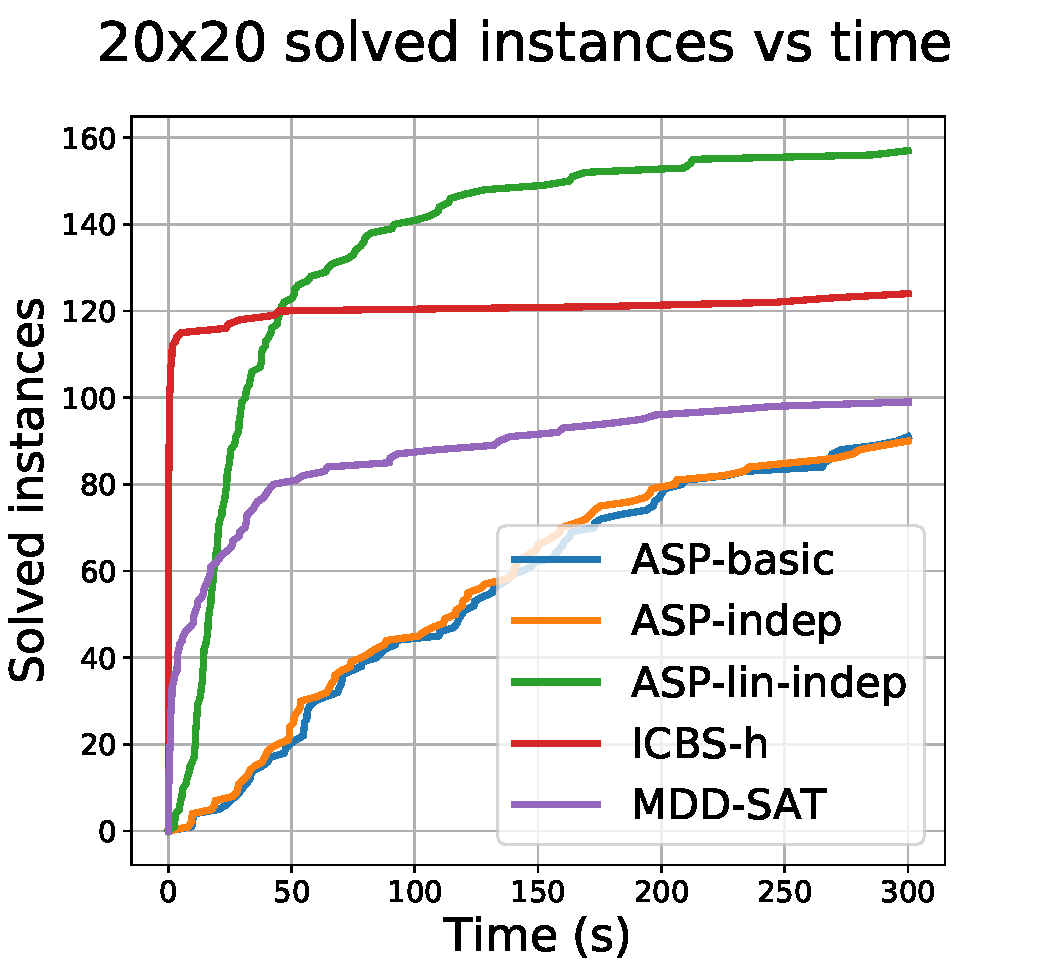
\includegraphics[width=0.24\textwidth]{graphs/20x20runtime.pdf}
    \caption{Success rate and number of instances solved versus time on $8\times 8$ and $20\times 20$ grids.}

    \label{fig_obs}
\end{figure*}

\begin{figure*}
    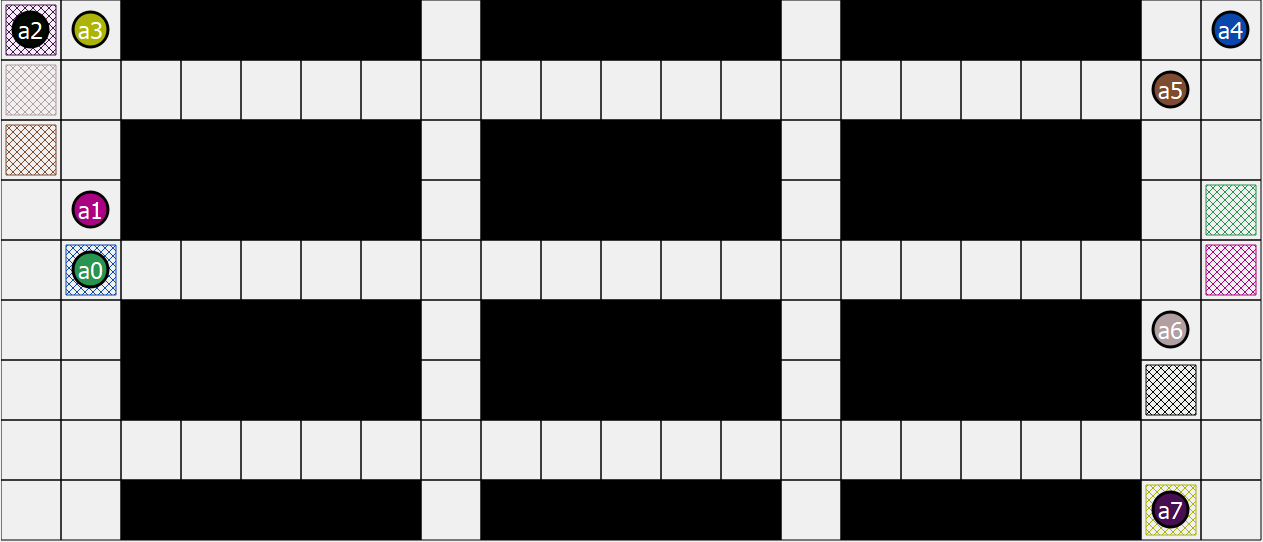
\includegraphics[width=0.45\textwidth]{graphs/warehouse.PNG}
    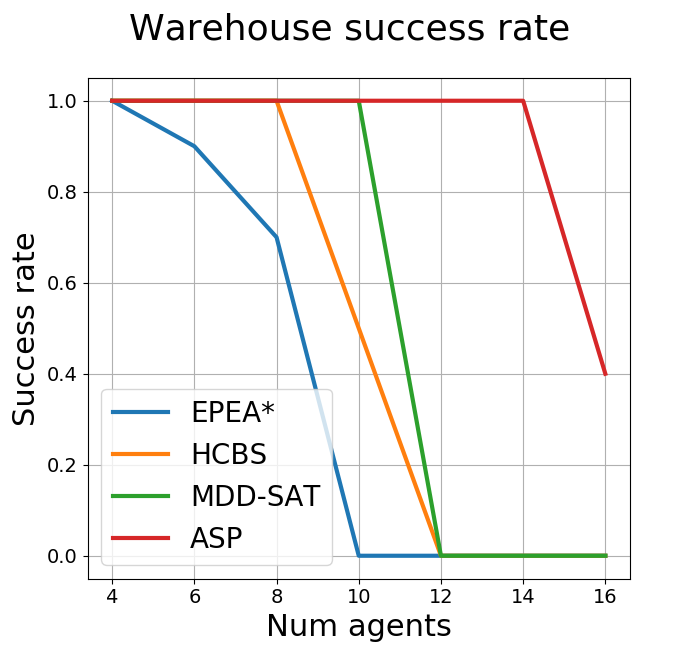
\includegraphics[width=0.24\textwidth]{graphs/warehousesucc.png}
    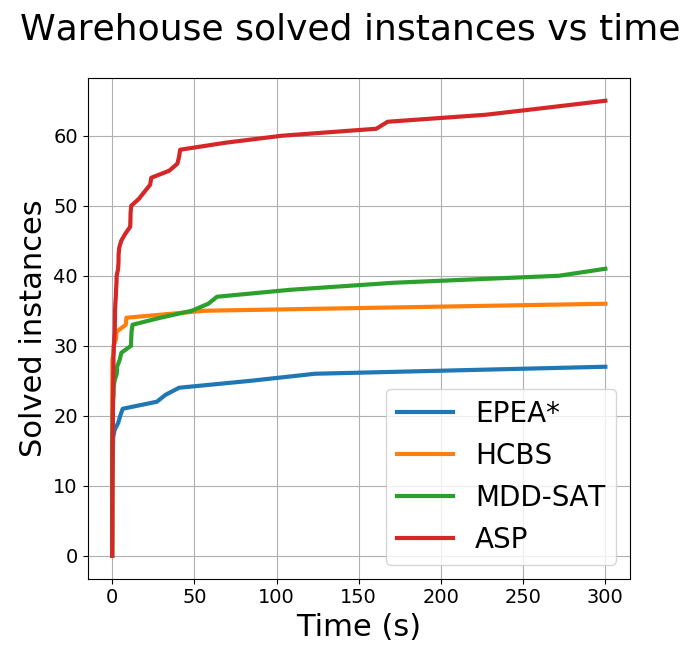
\includegraphics[width=0.24\textwidth]{graphs/warehouseruntime.png}
    \caption{Warehouse problem example and results}
    \label{fig_ware}
\end{figure*}

The objective of our empirical evaluation was to compare the performance of the different variants of our translation against representatives of search-based and SAT-based solvers. We compared to the publicly available SAT-based solver MDD-SAT \cite{Surynek14} (enc=mdd), and the search-based solvers EPEA* \cite{Goldenberg14}, and ICBS-h \cite{FelnerLB00KK18}. Our evaluation is focused on relatively small grids since grounding time grows too much for larger grids (e.g., $512\times 512$), making the approach impractical.


We compared different four different encodings: ASP-basic is a basic encoding that uses quadratic conflict resolution and grid-dependent penalties. ASP-indep uses quadratic conflict resolution and grid-independent penalties. Finally, ASP-lin-indep uses linear conflict resolution and grid-independent penalties. \jb{\textbf{REVISAR LOS NOMBRES Y AGREGAR EL QUE FALTA}}

The code used for our implementation was written in Python 3.7 using Clingo 5.3 \cite{GebserKKS14} for the ASP solver. Clingo was run with 4 threads in \textit{parallel-mode}, and using \textit{usc} as the optimization strategy. All algorithms we compared with were obtained from their authors.

All experiments were run on a 3.40GHz Intel Core i5-3570K with 8GB of memory running Linux. We set a runtime limit of 5 minutes for all problems.


\subsection{Obstacle-Free $N\times N$ Grids} First, we experimented on $N\times N$ obstacle-free grids with sizes $N\in\{8,16,32,64\}$. For each grids we generated $10$ instances for each number of agents $k\in \{2,4, \ldots N^2 -2 \}$. The agents' initial and goal cells were randomly placed.


In figure we show the \emph{breaking point}. of the thingy


\subsection{$N\times N$ Grids with Random Obstacles}
Next, we experimented on $8\times 8$ and $20\times 20$ randomly generated problems with 10\% obstacles. For $8\times8$ (resp.~$20\times 20$) we generate 150 (resp.~160) problems with the number of agents in $\{4,\dots,18\}$ (resp.~$\{20,22,\ldots,50\}$). Success rates, and number of problems solved versus time are shown in Figure ~\ref{fig_obs}.

In the $8\times8$ grids, as the number of agents increase, all our encodings outperform the other algorithms in terms of success rate. We also observe that our modifications to the basic encoding pay off substantially. We observe a substantial difference between our grid-dependent encoding and our grid-independent encoding.

For $20x20$ grids, we observe that our linear encoding solves almost all problems and substantially outperforms our quadratic (basic) encoding. We do not observe in this case an important impact of the grid-dependent encoding over grid-independent encoding.


\subsection{Warehouse experiments}
We experimented on a the warehouse grid shown in Figure~\ref{fig_ware}, used in the MAPF literature (e.g., \nbcite{FelnerLB00KK18}). We selected random initial and goal locations over the left and right borders of the grid. We generated $10$ instances for each number of agents $k\in \{4, \ldots, 16\}$.

\jb{\bf decir que usamos el mejor encoding encontrado en las grillas $n\times n$ acá}
\jb{\bf Decir que aquí quisimos probar dos de los modos de optimización en que funciona clingo para ver los posibles efectos. traducir el resto} Otro punto importante es el uso del método de USC con respecto a BB. USC parte con una solución costo mínimo que no necesariamente satisface los constraints, luego hace cambios hasta encontrar una solución que cumpla estos constraints. bb por otro lado primero encuentra una solución que satisface lo constraints y hace cambios a la solución hasta encontrar y demostrar una solución de costo mínimo. Debido a que normalmente la solución a los problemas en MAPF es más cercana a la solución óptima ignorando los conflictos es que USC muestra mejores resultados.

\jb{\bf hablar del beneficio de usar costToGo. Puedes dar un dato más duro, por ejemplo cuánto más rápido es o cuáles son los porcentajes}

Results show the benefits of our approach in this type of grids, where we outperform substantially the planners we compare with. Given the limited amount of free space on these grids, $|V|$ is smaller and thus our encoding is rather compact. These results also illustrate that our approach can cope nicely and more effectively than other approaches when the number of potential conflicts grow.
